
\textbf{جدول ثبت نتایج و نمودار برازش}
\vspace{1cm}
\begin{table}[htbp]
    \centering
    \renewcommand{\arraystretch}{1.2}
    \setlength{\tabcolsep}{14pt}
    \begin{latin}
        \begin{tabular}{c|c|c}
            \toprule
            \(h \pm \Delta h\)                        & \(\varphi \pm \Delta\varphi \) & \(\nu_0\pm \Delta\nu_0 \)         \\
            \midrule
            \qty{6.163 \pm 0.259 e-34}{\joule\second} & \qty{1.574\pm 0.102}{\volt}    & \qty{4.091 \pm 0.316 e14}{\hertz} \\
            \bottomrule
        \end{tabular}
    \end{latin}
    \caption{جدول ثبت نتایج}
\end{table}

\vspace{1cm}

\begin{figure}[!htbp]
    \centering
    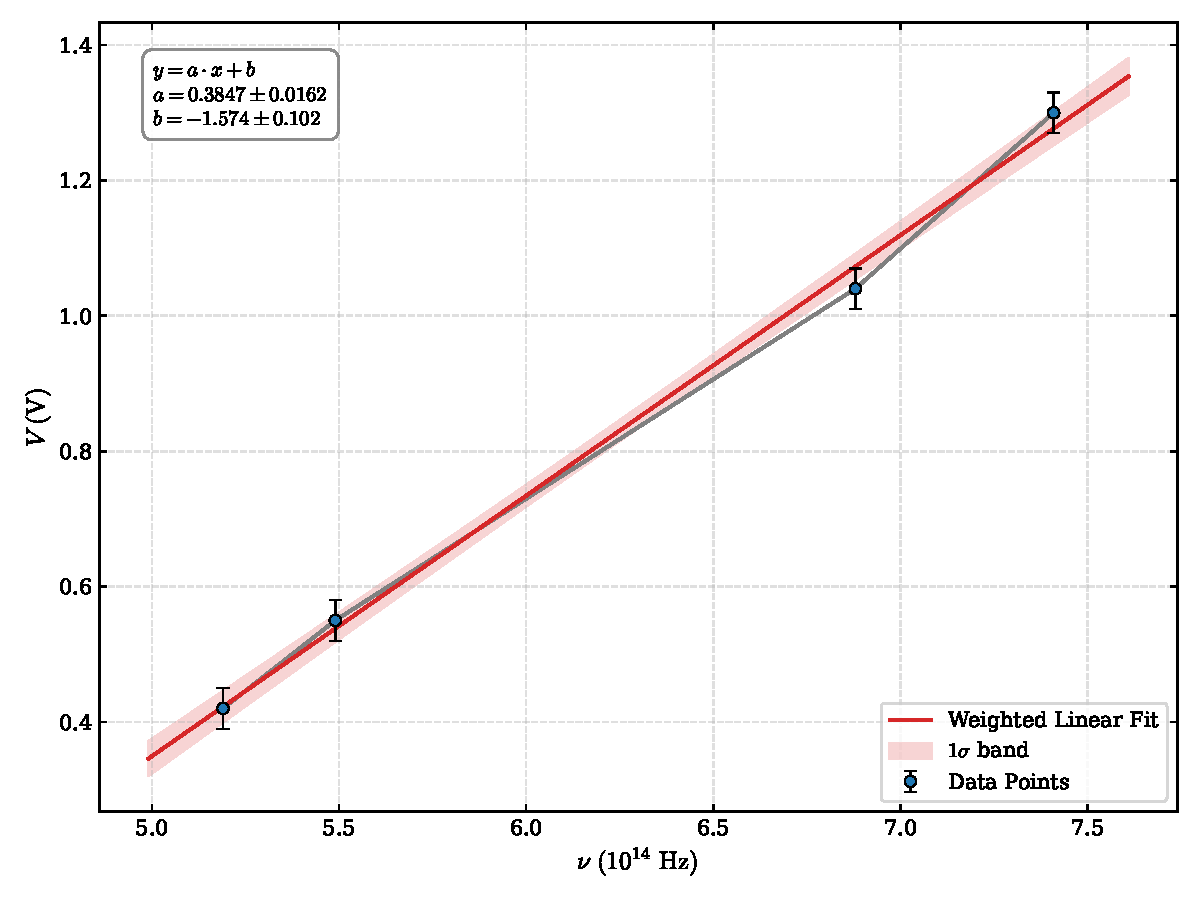
\includegraphics[width=0.9\textwidth]{figures/photoelectric.pdf}
    \caption{نمودار برازش داده های تجربی}
\end{figure}